% !TeX program = lualatex
% Lualatex is important to render Fira fonts; with pdflatex it's just the regular one
\documentclass[12pt]{beamer}

\usetheme{metropolis}
\usepackage{appendixnumberbeamer}

% adjust the background to be completely white
\setbeamercolor{background canvas}{bg=white}

\usepackage{booktabs}
\usepackage[scale=2]{ccicons}

\usepackage{pgfplots}
\usepgfplotslibrary{dateplot}

% typeset mathematics on serif
\usefonttheme[onlymath]{serif}

% better bibliography using biber as backend
\usepackage[natbib=true,backend=biber,style=authoryear-icomp,maxbibnames=30,maxcitenames=2,uniquelist=false,giveninits=true,doi=false,url=false,dashed=false,isbn=false]{biblatex}
% shared bibliogrphy
\addbibresource{../dl4nlp-bibliography.bib}
% disable "ibid" for repeated citations
\boolfalse{citetracker}

% TODOs
\usepackage{todonotes}
\let\todox\todo
\renewcommand\todo[1]{\todox[inline]{#1}}

\definecolor{76abdf}{RGB}{118, 171, 223}

\setbeamercolor{frametitle}{bg=76abdf, fg=white}

\usepackage{xspace}
\newcommand{\themename}{\textbf{\textsc{metropolis}}\xspace}

% POS tags
\newcommand*\POS[1]{\textsubscript{\texttt{#1}}} % tag with part of speech

% parse tree
\usepackage{qtree}

% NNEts
\usepackage{tikz}
\usetikzlibrary{matrix, positioning, calc}

\tikzset{
	neuron/.style={
		draw,
		circle,
		inner sep=0pt,
		minimum width=0.75cm
	},
	layer/.style={
		matrix of nodes,
		nodes={neuron},
		row sep={between origins, 1.2cm}, %1.5cm in general, 2.5cm for backprop task
		nodes in empty cells
	}
}




\title{Deep Learning for Natural Language Processing}
\subtitle{Lecture 1 -- Kick-off}
\date{April 12, 2021}
\author{Dr.\ Ivan Habernal}
\institute{Trustworthy Human Language Technologies  \hfill 
\includegraphics[height=.8cm]{img/logo-trusthlt.pdf} \\
Department of Computer Science\\
Technical University of Darmstadt \hfill \texttt{www.trusthlt.org} }
%\titlegraphic{\hfill }

\begin{document}

\maketitle


\begin{frame}{Table of contents}
	

  \setbeamertemplate{section in toc}[sections numbered]
  \tableofcontents[hideallsubsections]
\end{frame}

\section{Administrative course issues}

\begin{frame}{Learning Goals}
	
After completing this course, you are able to 

\begin{itemize}
\item  explain the basic concepts of \textbf{neural networks and deep learning},
\item explain the concept of \textbf{word embeddings}, train word embeddings and use them for solving NLP problems,
\item understand and describe neural network architectures that are used to tackle classical \textbf{NLP problems} such as text/sentence classification and sequence tagging,
\item \textbf{implement} neural networks for NLP problems using existing libraries in Python
\end{itemize}

\end{frame}


\begin{frame}[fragile]{General Information}

\metroset{block=fill}
\begin{block}{Teaching material}
Lectures, exercises/submissions etc. can be found in Moodle
\end{block}	

\end{frame}


\begin{frame}{Resources}
	
\begin{itemize}
\item This lecture is mainly based on recent papers from top NLP conferences
	\begin{itemize}
		\item Deep Learning is still evolving quickly
		\item Knowledge gets outdated
	\end{itemize}
\end{itemize}

\end{frame}


\begin{frame}{Useful Additional Resources}

Ian Goodfellow, Yoshua Bengio, and Aaron Courville: Deep Learning, MIT Press (\textbf{freely available} online book!)

Stanford Lecture by Richard Socher: \emph{Deep Learning for Natural Language Processing cs224d} (look it up on YouTube)
	
Yoav Goldberg: Neural Network Methods for Natural Language Processing (not free)

Marc Peter Deisenroth, A. Aldo Faisal, and Cheng Soon Ong: Mathematics for Machine Learning (\textbf{freely available} PDF!)
	
Jeremy Kun: A Programmer's Introduction to Mathematics (PDF "\textbf{Pay what you want}")

\end{frame}


\begin{frame}{Recommended Readings}

We provide literature for each topic of our course:

\begin{itemize}
	\item Even if you have very limited time, please do read the \textbf{mandatory part} -- we will assume that you know these works.
	\item The mandatory papers
%	(roughly one per week)
	will be ``prüfungsrelevant'' (relevant for the exam).
	\item We will ask one/two questions from the mandatory papers in the homeworks.
\end{itemize}

We \textbf{encourage} you to read the optional parts as well (listed in each lecture).

If you cannot find/access a publication $\to$ feel free to ask.

\end{frame}

\begin{frame}{Exercises and Homeworks (I)}
	
	\textbf{Exercises (EX)}
	\begin{itemize}
		\item Deepening and testing the understanding from the lecture
		\item Not graded
	%	\item The exercises will give you some practical experience and hands-on training of what you learned.
	%	\item You will learn to program neural nets, which we don't do/teach in the lecture.
	\end{itemize}
	
	\textbf{Homeworks (HW)}
	\begin{itemize}
		\item Practically applying your knowledge from the lecture (and exercises)
		\item Mostly programming + a bit of math and paper reading
		\item Submit in groups of two
		\item First homework will be published today
	\end{itemize}

	EX and HW organized by Jonas Rikowski
\end{frame}
\begin{frame}{Exercises and Homeworks (II)}
	
	\textbf{Questions}
	\begin{itemize}
		\item Moodle forums, Discord server
		\item Only for personal questions: Private Moodle message to the tutors
	\end{itemize}

	\colorbox{purple!10}{\textcolor{purple}{\textbf{To do after this lecture}}}
	\begin{enumerate}
		\item Read the exercise and homework \textbf{logistics} (PDF) on Moodle thoroughly
		\item Select your homework \textbf{group} on Moodle (deadline: April 22)
	\end{enumerate}

\end{frame}

\begin{frame}{Shared Task}

The shared task is organized by \textbf{Philipp Marquardt}
	
You will work on \textbf{Conversational AI}

You will work in groups of up to 3 people

You will develop a solution to the problem and then compete with other groups

Shared task is graded and gives up to 100 points. Grading is based on:

- Written report about your system (60 points)

- Your ranking compared to other teams -> better system, more points (30 points)

- A short presentation in the last class (10 points)


	
\end{frame}

\begin{frame}{Bonus System}

By submitting the homeworks and participating in the shared task, you can get a bonus of 0.3 (or 0.4) for the exam.

You need to reach $\geq$ \textbf{70\%}\footnote{subject to changes} of the summed homework and shared task points.

More details: $\to$ exercise and homework \textbf{logistics} on Moodle.

\end{frame}

\begin{frame}{Tutors}
	
Jonas Rikowski

Philipp Marquardt
	

If you have personal questions, contact them via moodle 
	
\end{frame}

\begin{frame}{Final Exam}


Save the date:

\todo{To be announced on Moodle}
%Friday, 9. August 2019, 14:00 -- 16:30

Register via TUCaN, see also:

\url{https://www.informatik.tu-darmstadt.de/de/studierende/
studienbuero/pruefungsan-und-abmeldung/}

Exam questions will be in English.
Answers may be in German or English.

\end{frame}

\begin{frame}{Final Exam: Resources Allowed}

Scope: Lecture, mandatory readings, and practice class

Final grade: Exam (100\%) + Bonus System

You may bring a dictionary to the exam, if neither German nor English is your first language.

You may bring a non-programmable calculator to the exam.

No other resources (books, lecture notes etc.) are allowed during the exam.
	
\end{frame}

\begin{frame}{Questions/Suggestions}

Any questions, suggestions?

Post a message in the Moodle forum or chat on Discord

If that doesn‘t help: Write an E-Mail to the tutors or make an appointment with them

If that doesn‘t help also: Write an email to me	
\end{frame}


\section{The TrustHLT Group}

\begin{frame}{Trustworthy Human Language Technologies}


\includegraphics[height=.8cm]{img/logo-trusthlt.pdf} \hfill \texttt{www.trusthlt.org}

\bigskip

- Privacy-preserving NLP (differential privacy; deep learning; representation learning; graph networks)

- Argument mining "that matters" (legal argument mining; ethical argumentation)

\bigskip

Master thesis? Get in touch!
	
\end{frame}


\section{Deep Learning for Natural Language Processing}

\begin{frame}{Deep Learning for Natural Language Processing}
	
	
Deep Learning = neural networks, sub-field of machine learning

NLP = Analysis of language
	
\end{frame}

\begin{frame}{History of Deep Learning 1}

Early booming (1950s -- early 1960s)

\begin{itemize}
	\item Rosenblatt (1958) -- Perceptron
	\item Widrow and Hoff (1960, 1962) --  Learning rule based on gradient descent
\end{itemize}

Setback (mid 1960s late 1970s)

\begin{itemize}
	\item Serious problems with perceptron model (Minsky’s book 1969)
	\item Can’t even represent simple functions
\end{itemize}


Renewed enthusiasm (1980s)

\begin{itemize}
	\item New techniques (Backpropagation for “deep nets”)
\end{itemize}

\end{frame}


\begin{frame}{History of Deep Learning 2}
	
Out-of-fashion -- again (1990s to mid 2000s)

\begin{itemize}
	\item Other techniques were considered superior and more understandable; Support Vector Machines, Integer linear programming, etc.
	\item So much out of fashion, some good CS journals immediately rejected papers on neural networks without review (as reported by Geoffrey Hinton)
	\item Played no role in top NLP conferences
\end{itemize}

Since mid 2000: huge progress for “deep learning”

\begin{itemize}
	\item Hinton and Salakhutdinov (2006): one can actually train deep nets
	\item Since ~2013: Word embeddings, work of Mikolov et al. 
\end{itemize}

\end{frame}

\begin{frame}{History of Deep Learning 3}
	
Since mid 2010: huge progress for “deep learning”

Why?
\begin{itemize}
	\item More data
	\item Faster computers, better hardware (GPU)
	\item Unsupervised pre-training
	\item Better optimization techniques, better understanding of the approaches, …
\end{itemize}
	
\end{frame}


\begin{frame}{Deep learning in NLP}
	
Occurrences of “neural” and “network” in titles in the ACL Anthology


\begin{figure}
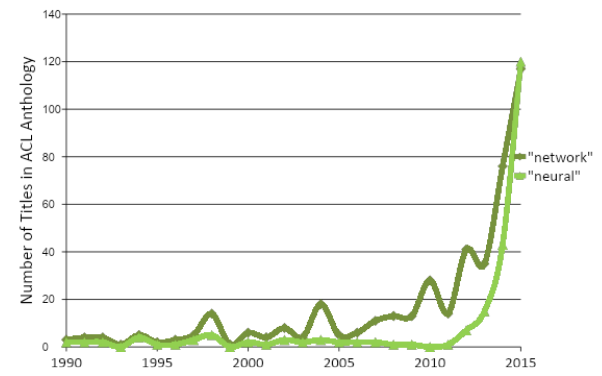
\includegraphics[width=0.7\linewidth]{img/screenshot_2021-03-24_15-06-54}	
\end{figure}
	
\end{frame}


\begin{frame}{DL Example: Machine translation}
\begin{figure}
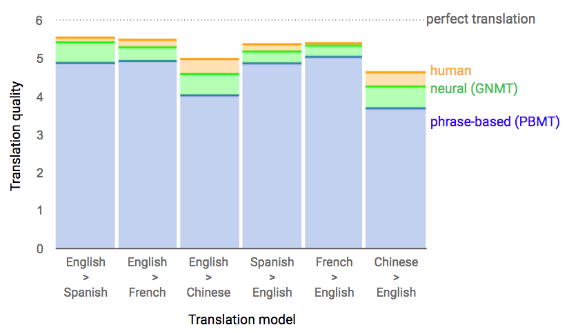
\includegraphics[width=0.9\linewidth]{img/screenshot_2021-03-24_15-09-30}
\end{figure}
	
\end{frame}

\begin{frame}{Not everything works!}
Depending on characteristics of your task, traditional approaches may still be preferable or superior

\begin{itemize}
	\item Neural nets seem to particularly excel on “difficult” tasks, less on simple tasks (task difficulty)
	\item Other factors such as training data size may play a crucial role	
\end{itemize}

Neural Networks are also prone to fooling

\begin{figure}
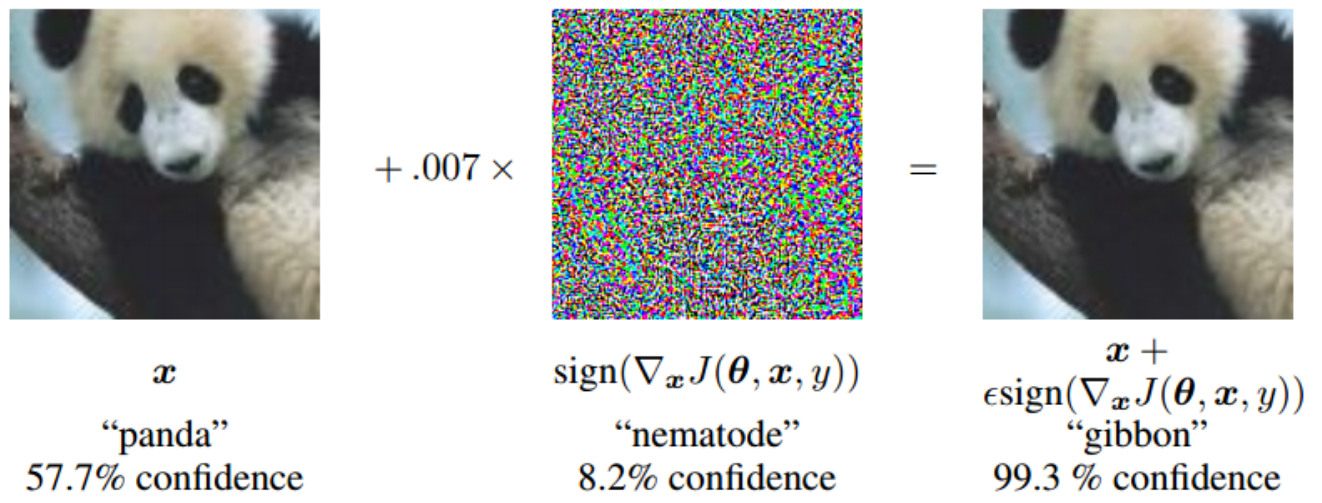
\includegraphics[width=0.6\linewidth]{img/screenshot_2021-03-24_15-12-45.png}
\end{figure}

\end{frame}


\begin{frame}{Examples of low-level NLP problems/tasks}

Sequence tagging

\begin{itemize}
	\item POS-tagging (part of speech)
\end{itemize}


	
\begin{exampleblock}{Example}
	Time flies   like   an   arrow.\\Fruit   flies   like   a   banana.
\end{exampleblock}

\bigskip

\begin{exampleblock}{Example}
		Time\POS{NN} flies\POS{VBZ}  like\POS{IN}   an\POS{DT}   arrow\POS{NN}.		\\ Fruit\POS{NN}   flies\POS{NN}   like\POS{VB}   a\POS{DT}   banana\POS{NN}.
\end{exampleblock}

\begin{footnotesize}
IN = Preposition or subordinating conjunction (conjunction here); VBZ = Verb, 3rd person singular present; DT = determiner; NN = singular noun
\end{footnotesize}

\end{frame}


\begin{frame}{Low-level NLP problems/tasks}
	
Sequence tagging

\begin{itemize}
	\item POS-tagging (part of speech)
\end{itemize}

Structure prediction
\begin{itemize}
	\item Chunking/Parsing
\end{itemize}

\begin{columns}[T,onlytextwidth]
\column{0.5\textwidth}

\begin{exampleblock}{Example}
\begin{scriptsize}
\Tree
[.S
	[.NP
		[.NN
			[ Time ]
		]
	]
	[.VP
		[.VBZ
			[ flies ]
		]
		[.PP
			[.IN
				[ like ]
			]
		]
		[.NP
			[.DT
				[ an ]
			]
			[.NN
				[ arrow ]
			]
		]
	]
]
\end{scriptsize}
\end{exampleblock}

\column{0.5\textwidth}

\begin{exampleblock}{Example}
	\begin{scriptsize}
\Tree
[.S
	[.NP
		[.NN
			[ Fruit ]
		]
		[.NN
			[ flies ]
		]
	]
	[.VP
		[.VB
			[ like ]
		]
		[.NP
			[.DT
				[ a ]
			]
			[.NN
				[ banana ]
			]
		]
	]
]
\end{scriptsize}
\end{exampleblock}
\end{columns}
	
\end{frame}


\begin{frame}{Examples of low-level NLP problems/tasks}
	
Sequence tagging

\begin{itemize}
	\item POS-tagging (part of speech)
\end{itemize}

Structure prediction
\begin{itemize}
	\item Chunking/Parsing
\end{itemize}


Semantics
\begin{itemize}
	\item Word sense disambiguation
\end{itemize}

	
	\begin{exampleblock}{Example}
		Time flies   like   an   arrow. \hfil Fruit   flies   like   a   banana. \\
		
\includegraphics[width=0.3\linewidth]{img/screenshot_2021-03-24_16-49-31.png} \hspace{5.5em}
		
\includegraphics[width=0.3\linewidth]{img/screenshot_2021-03-24_16-49-45.png}
	\end{exampleblock}
	
\end{frame}


\begin{frame}{High-level NLP tasks}


\begin{itemize}
	\item Information Extraction
	\begin{itemize}
		\item search, event detection, textual entailment
	\end{itemize}
	\item Writing Assistance 
	\begin{itemize}
		\item spell checking, grammar checking, auto-completion
	\end{itemize}
	\item Text Classification
	\begin{itemize}
		\item spam, sentiment, author, plagiarism
	\end{itemize}
	\item Natural language understanding 
	\begin{itemize}
		\item metaphor analysis, argumentation mining, question-answering
	\end{itemize}
	\item Natural language generation
	\begin{itemize}
		\item summarization, tutoring systems, chat bots
	\end{itemize}
	\item Multilinguality
	\begin{itemize}
		\item machine translation, cross-lingual information retrieval
	\end{itemize}
\end{itemize}

	
\end{frame}


\begin{frame}{Example: Named Entity Recognition (NER) 1}

\begin{exampleblock}{Example}
"... chancelor\POS{O} Angela\POS{B-PER} Merkel\POS{I-PER} said\POS{O} ..."
\end{exampleblock}

"BIO"-tagging
\begin{itemize}
	\item \texttt{B} = Begin of entity, e.g., \texttt{B-PER} (person), \texttt{B-LOC} (location)
	\item \texttt{I} = "Inside" entity, e.g, \texttt{I-PER}, \texttt{I-LOC}
	\item \texttt{O} = Other (no entity)
\end{itemize}
	
\end{frame}

\begin{frame}{Traditional feature engineering}
	
	\begin{exampleblock}{Example -- determining tag for \emph{Angela}}
		"... chancelor\POS{O} \textbf{Angela}\POS{B-PER} Merkel\POS{I-PER} said\POS{O} ..."
	\end{exampleblock}
	
Each token is represented by a feature vector

\begin{table}
	\small
%	\caption{Largest cities in the world (source: Wikipedia)}
	\begin{tabular}{@{} lr @{}}
		\toprule
		Feature type & Value \\
		\midrule
		uppercase & 1\\
		is Noun & 1\\
		previousWord DET& 0\\
		previousWord uppercased& 0\\
		following word N & 1\\
		following word uppercased & 1 \\
		... & ... \\
		\bottomrule
	\end{tabular}
\end{table}

\end{frame}

\begin{frame}{Traditional feature engineering (cont.)}
	
	\begin{exampleblock}{Example -- determining tag for \emph{Merkel}}
		"... chancelor\POS{O} Angela\POS{B-PER} \textbf{Merkel}\POS{I-PER} said\POS{O} ..."
	\end{exampleblock}
	
	Each token is represented by a feature vector
	
	\begin{table}
		\small
		%	\caption{Largest cities in the world (source: Wikipedia)}
		\begin{tabular}{@{} lr @{}}
			\toprule
			Feature type & Value \\
			\midrule
			uppercase & 1\\
			is Noun & 1\\
			previousWord DET& 0\\
			previousWord uppercased& 1\\
			following word N & 0\\
			following word uppercased & 0 \\
			... & ... \\
			\bottomrule
		\end{tabular}
	\end{table}
	
\end{frame}

\begin{frame}{Traditional feature engineering (cont.)}
	
	Word specific features
	
	\begin{itemize}
		\item previous word is minister
		\item previous word is chancellor
		\item previous word is president
		\item previous word is company
		\item previous word is product
		\item following word is says
		\item following word is declares
		\item following word is claims
	\end{itemize}
	
	Problem: Similar words are represented as distinct features.
\end{frame}

\begin{frame}{DL for NER}
		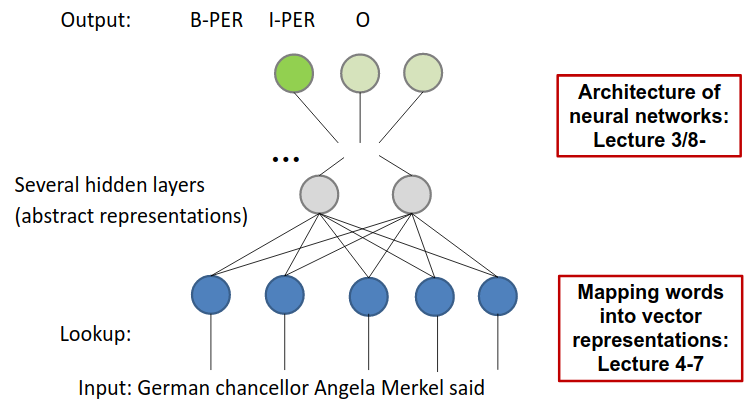
\includegraphics[width=\linewidth]{img/screenshot_2021-03-24_17-19-10.png}
\end{frame}


\section{Perceptron}

\begin{frame}{Origins}
	
‘Simplest’ form of a neural network

Perceptron is an algorithm for learning a binary classifier

Introduced by McCulloch and Pitts (1943) and Frank Rosenblatt (1958)

\begin{figure}
	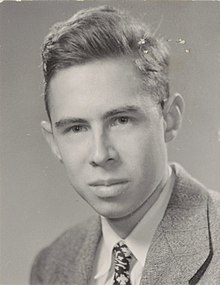
\includegraphics[width=0.2\linewidth]{img/220px-Rosenblatt_21.jpg}
	\caption{Frank Rosenblatt; Source: Wikipedia}	
\end{figure}
	

\end{frame}



\begin{frame}{Perceptron in detail}
	
	
	
	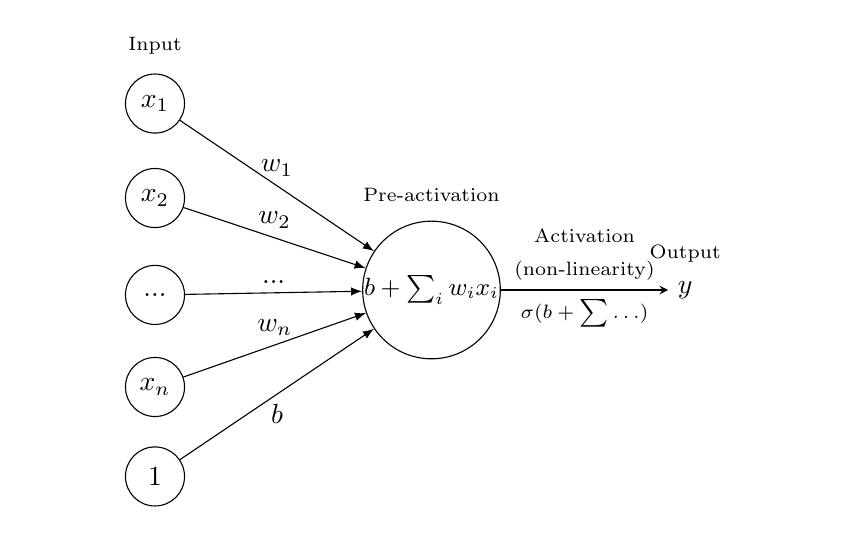
\begin{tikzpicture}
	\begin{scope}[node distance=2cm] % 2cm in general, 3.5cm for backprop task
	\matrix[layer] (input) {
		$x_1$\\
		$x_2$\\
		...\\
		$x_n$\\
		$1$\\
	};
	
%	\matrix[layer, right=of input] (dense1) {
%	\matrix[layer] (dense1) {		
%		$q_1$ \\
%		$q_2$ \\
%		$q_3$ \\
%	};
	
	\matrix[layer, right=of input] (output) {
		\small
		$b + \sum_{i}  w_i  x_i$ \\
	};
	
	% dense layer connections
	\begin{scope}[thin, ->, >=latex]
	% input -> dense1
%	\foreach \inputnode in {1,2,3,4} {
%		\foreach \hiddennode in {1,2,3} {
%			\draw (input-\inputnode-1) -- (dense1-\hiddennode-1);
%		}
%	}

	\draw (input-1-1) -- (output-1-1) node[midway,above]{$w_1$};
	\draw (input-2-1) -- (output-1-1) node[midway,above]{$w_2$};
	\draw (input-3-1) -- (output-1-1) node[midway,above]{...};
	\draw (input-4-1) -- (output-1-1) node[midway,above]{$w_n$};
	\draw (input-5-1) -- (output-1-1) node[midway,below]{$b$};
	
	% dense -> output
%	\foreach \done in {1,2,3} {
%		\draw (dense1-\done-1) -- (output-1-1);
%	}
	\end{scope}
	
	% matrix labels
%	\node at ($(input)!0.5!(dense1)$) {$\mathbf{V}$};
%	\node at ($(dense1)!0.5!(output)$) {$\mathbf{W}$};
	
	\node[right=of output] (final) {$y$};

	% to the output
	\draw [-stealth] (output-1-1) -- (final) node[midway,below] {
		\scriptsize $\sigma(b + \sum \dots)$
	}
	node[midway,above,align=center] {\scriptsize Activation\\ \scriptsize (non-linearity)};
	
	% layer descriptions
	\begin{scope}[every node/.style={align=center,text width=3cm}]
	\node[above=0cm of input] (inputdesc) {\scriptsize Input};
	\node[above=0cm of output] (outputdesc) {\scriptsize Pre-activation};
	\node[above=0cm of final] (finaldesc) {\scriptsize Output};
	

	
%	\node[above=0cm of dense1] (dense1_descr) {$\mathbf{q}$\\ $\sigma_\mathbf{q}=$ sigmoid}; %0cm in general, 1cm for backprop task
%	\node at (dense1_descr -| input) {$\mathbf{x}$};
%	\node at (dense1_descr -| output) {$\mathbf{y}$\\$\sigma_\mathbf{y}=\tanh$};
	\end{scope}
	\end{scope}
	\end{tikzpicture}
	
	
\end{frame}

\begin{frame}{Formal description}
	
Given

- weight vector and bias $\mathbf{w} \in \mathbb{R}^n$, $b \in \mathbb{R}$

- non-linear function $\sigma : \mathbb{R} \to \mathbb{R}$

Input to network

- Input vector $\mathbf{x} \in \mathbb{R}^n$

- and constant $1$

Output unit

- Input: $\underbrace{\mathbf{x} \cdot \mathbf{w}}_{\text{Dot product}} + b = \sum_{i = 1}^{n} (w_i x_i) + b$

- Output: $\sigma (\mathbf{x} \cdot \mathbf{w} + b)$
	
\end{frame}


\begin{frame}{Simplification}
	
Given

- weight vector (incl. bias term) $\mathbf{w} \in \mathbb{R}^{(n + 1)}$

- non-linear function $\sigma : \mathbb{R} \to \mathbb{R}$

Input to network

- Input vector $\tilde{\mathbf{x}} \in \mathbb{R}^{(n+1)} = (\mathbf{x} \quad 1)$ 


Output unit

- Input: $\tilde{\mathbf{x}} \cdot \mathbf{w} = \sum_{i = 1}^{n} w_i x_i$

- Output: $\sigma (\tilde{\mathbf{x}} \cdot \mathbf{w})$
	
	

\end{frame}


\begin{frame}{Optimization problem}
	
Perceptron is the function $f : \mathbb{R}^{n+1} \to \mathbb{R}$ where $f(\mathbf{x}; \mathbf{w}) = \sigma (\tilde{\mathbf{x}} \cdot \mathbf{w})$

Vector $\mathbf{w}$ are the parameters we want to "learn"

Training data is a set of $N$ examples

$$\{(\mathbf{x}_1, y_1),  \dots, (\mathbf{x}_N, y_N) \}$$

We want to minimize "the difference" between the true $y$-s and what our network outputs

$$
\min_{\mathbf{w}} \sum_{j = 1}^{N} (f(\mathbf{x}; \mathbf{w}) - y_j )^2
$$
	
	
\end{frame}


\begin{frame}{How do we minimize the loss function?}
	
$$
\min_{\mathbf{w}} \sum_{j = 1}^{N} (f(\mathbf{x}; \mathbf{w}) - y_j )^2
$$

We will employ a general optimization technique called \emph{(stochastic) gradient descend}; more in Lectures 2 \& 3


	
\end{frame}


\begin{frame}{Perceptron for binary classification and decision surface}
	

Perceptron uses a simple threshold function for decisions

$$
\sigma(z) =
\begin{cases}
0  & \quad \text{if } z < 0\\
1  & \quad \text{if } z \geq 0
\end{cases}
$$

Example 2-D input; 2 neurons (= features) and bias; ($\mathbf{x} \in \mathbb{R}^2)$

the decision boundary is a straight line $y = az + b$

	
\end{frame}

\begin{frame}{Linear separation}


\begin{figure}
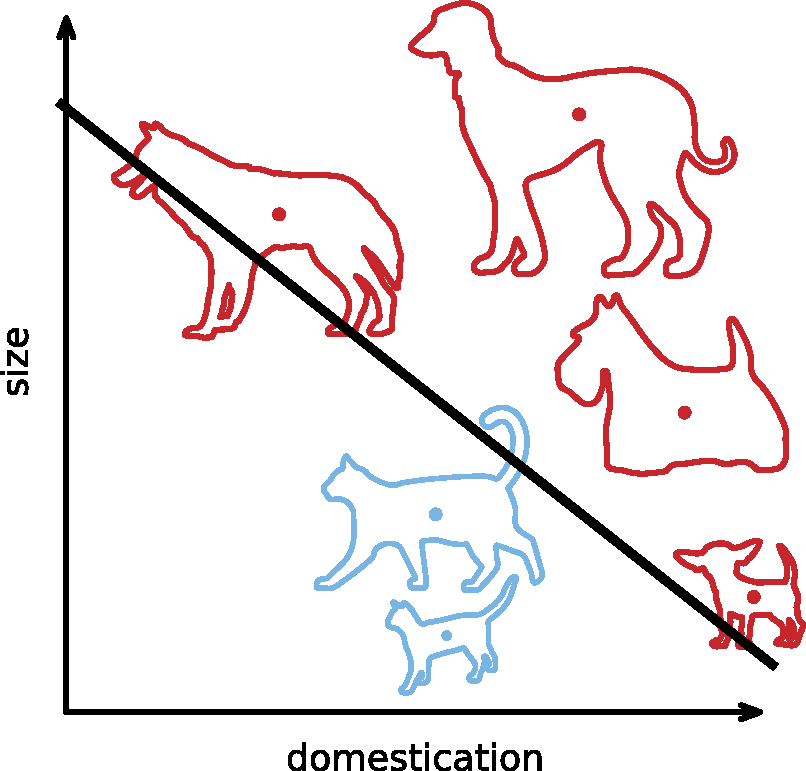
\includegraphics[width=0.5\linewidth]{img/Perceptron_example_wikipedia.pdf}	
\caption{Linear boundary of perceptron\footnote{\tiny \url{https://en.wikipedia.org/wiki/Perceptron}}}
	
\end{figure}	

\end{frame}

\begin{frame}{What a perceptron can do}
	
Linear separability

Let $X_0$ and $X_1$ be two sets of points in an $n$-dimensional Euclidean space.
Then $X_0$ and $X_1$ are \emph{linearly separable} if there exist $n + 1$ real numbers $w_1, \dots, w_{n + 1}$ such that every point $\mathbf{x} \in X_0$ satisfies $\tilde{\mathbf{x}} \cdot \mathbf{w} > 0$ and every point $\mathbf{x} \in X_1$ satisfies $\tilde{\mathbf{x}} \cdot \mathbf{w} \leq 0$
	
\end{frame}

\begin{frame}{What a perceptron cannot do}
	
\begin{figure}
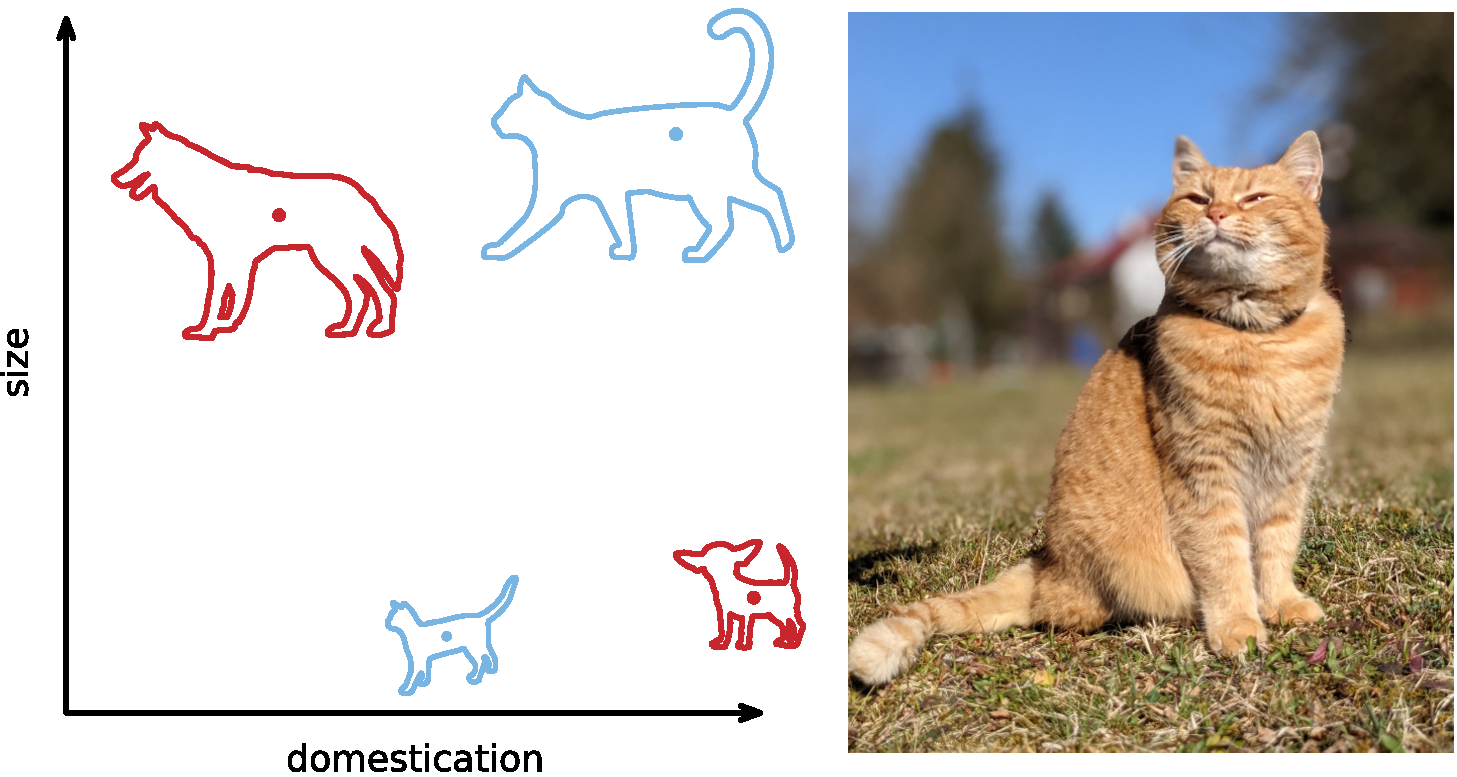
\includegraphics[width=0.7\linewidth]{img/Perceptron_example_wikipedia_xor.pdf}
\caption{Examples of XOR (exclusive or)\footnote{\tiny \url{https://en.wikipedia.org/wiki/Perceptron}}}
\end{figure}
	
\end{frame}



\section{Neural Network Principles}


\begin{frame}{Multiple output nodes}
	
\begin{columns}[T,onlytextwidth]
	\column{0.5\linewidth}

	% move to the left by 3 em
	\hspace{-3em}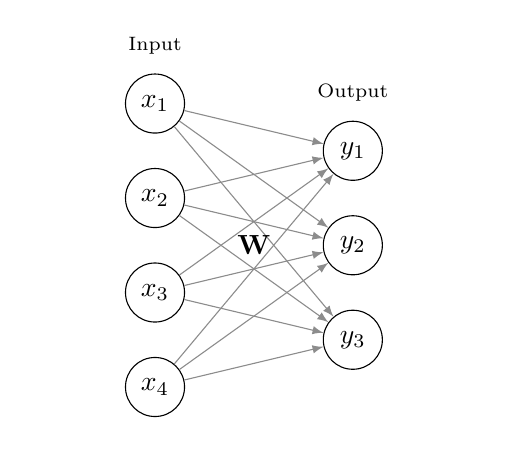
\begin{tikzpicture}
	\begin{scope}[node distance=1.5cm] % 2cm in general, 3.5cm for backprop task
	\matrix[layer] (input) {
		$x_1$\\
		$x_2$\\
		$x_3$\\
		$x_4$\\
	};
	
	\matrix[layer, right=of input] (output) {
		$y_1$ \\
		$y_2$ \\
		$y_3$ \\		
	};
	
	% dense layer connections
	\begin{scope}[thin, black!45, ->, >=latex]
	% input -> output
	\foreach \in in {1,2,3,4} {
		\foreach \done in {1,2,3} {
			\draw (input-\in-1) -- (output-\done-1);
		}
	}

	\end{scope}
	
	
	% matrix labels
	\node at ($(input)!0.5!(output)$) {$\mathbf{W}$};
	

	% layer descriptions
	\begin{scope}[every node/.style={align=center,text width=3cm}]
	\node[above=0cm of input] (inputdsc) {\scriptsize Input};
	\node[above=0cm of output] (outputdsc) {\scriptsize Output};
	\end{scope}

	\end{scope}
	\end{tikzpicture}
	
	\column{0.5\linewidth}
	
	- Previously for 1-D output: a dot product $\mathbf{x} \cdot \mathbf{w}$
	
	- Now matrix multiplication $\mathbf{x} \times \mathbf{W}$
	
	- Weights are in a matrix $\mathbf{W}$
	
	- $\mathbf{x}$ is a row vector
	
	- Each column in $\mathbf{W}$ corresponds to weights of $j$-th output $y_j$

\end{columns}

\end{frame}


\begin{frame}{Hidden layers}
	
Multiple hidden units/hidden layer(s)

		
		% move to the left by 3 em
		\hspace{-3em}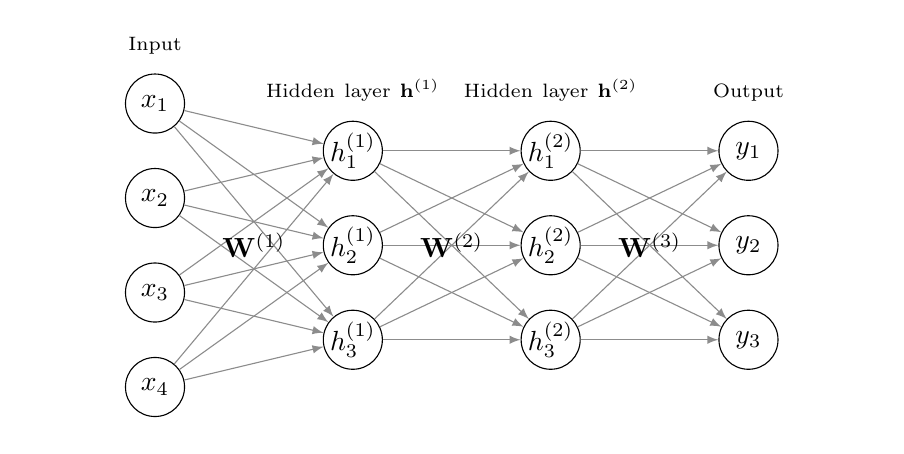
\begin{tikzpicture}
		\begin{scope}[node distance=1.5cm] % 2cm in general, 3.5cm for backprop task
		\matrix[layer] (input) {
			$x_1$\\
			$x_2$\\
			$x_3$\\
			$x_4$\\
		};
	
		\matrix[layer, right=of input] (hidden1) {
			$h_1^{(1)}$ \\
			$h_2^{(1)}$ \\
			$h_3^{(1)}$ \\		
		};
	
		\matrix[layer, right=of hidden1] (hidden2) {
			$h_1^{(2)}$ \\
			$h_2^{(2)}$ \\
			$h_3^{(2)}$ \\		
		};
			
		\matrix[layer, right=of hidden2] (output) {
			$y_1$ \\
			$y_2$ \\
			$y_3$ \\		
		};
		
		% dense layer connections
		\begin{scope}[thin, black!45, ->, >=latex]
		% input -> hidden
		\foreach \in in {1,2,3,4} {
			\foreach \done in {1,2,3} {
				\draw (input-\in-1) -- (hidden1-\done-1);
			}
		}
	
	
		\foreach \in in {1,2,3} {
			\foreach \done in {1,2,3} {
				\draw (hidden1-\in-1) -- (hidden2-\done-1);
			}
		}

		% input -> hidden
		\foreach \in in {1,2,3} {
			\foreach \done in {1,2,3} {
				\draw (hidden2-\in-1) -- (output-\done-1);
			}
		}

		
		\end{scope}
		
		
		% matrix labels
		\node at ($(input)!0.5!(hidden1)$) {$\mathbf{W}^{(1)}$};
		\node at ($(hidden1)!0.5!(hidden2)$) {$\mathbf{W}^{(2)}$};
		\node at ($(hidden2)!0.5!(output)$) {$\mathbf{W}^{(3)}$};
		
		
		% layer descriptions
		\begin{scope}[every node/.style={align=center,text width=3cm}]
		\node[above=0cm of input] (inputdsc) {\scriptsize Input};
		\node[above=0cm of hidden1] (hiddendsc) {\scriptsize Hidden layer $\mathbf{h}^{(1)}$};
		\node[above=0cm of hidden2] (hiddendsc) {\scriptsize Hidden layer $\mathbf{h}^{(2)}$};		
		\node[above=0cm of output] (outputdsc) {\scriptsize Output};
		\end{scope}
		
		\end{scope}
		\end{tikzpicture}
		
This architecture is known as \textbf{Multi-Layer Perceptron (MLP)}.

	
\end{frame}



%
%\begin{frame}{Perceptron in detail}
%
%\begin{tikzpicture}
%\begin{scope}[node distance=2cm] % 2cm in general, 3.5cm for backprop task
%\matrix[layer] (input) {
%	$x_1$\\
%	$x_2$\\
%	$x_1$\\
%	$x_2$\\
%};
%
%\matrix[layer, right=of input] (dense1) {
%	$q_1$ \\
%	$q_2$ \\
%	$q_3$ \\
%};
%
%\matrix[layer, right=of dense1] (output) {
%	$y_1$ \\
%};
%
% dense layer connections
%\begin{scope}[thin, black!45, ->, >=latex]
% input -> dense1
%\foreach \in in {1,2,3,4} {
%	\foreach \done in {1,2,3} {
%		\draw (input-\in-1) -- (dense1-\done-1);
%	}
%}
%
% dense -> output
%\foreach \done in {1,2,3} {
%	\draw (dense1-\done-1) -- (output-1-1);
%}
%\end{scope}
%
%% matrix labels
%\node at ($(input)!0.5!(dense1)$) {$\mathbf{V}$};
%\node at ($(dense1)!0.5!(output)$) {$\mathbf{W}$};
%
% layer descriptions
%\begin{scope}[every node/.style={align=center,text width=3cm}]
%\node[above=0cm of dense1] (dense1_descr) {$\mathbf{q}$\\ $\sigma_\mathbf{q}=$ sigmoid}; %0cm in general, 1cm for backprop task
%\node at (dense1_descr -| input) {$\mathbf{x}$};
%\node at (dense1_descr -| output) {$\mathbf{y}$\\$\sigma_\mathbf{y}=\tanh$};
%\end{scope}
%\end{scope}
%\end{tikzpicture}
%
%\end{frame}


\begin{frame}{Computations in detail}


$$
\mathbf{h}^{(1)} = \sigma(\mathbf{x} \mathbf{W}^{(1)} + b)
$$
	
	where $\sigma()$ is applied element-wise, for example

	 $\mathbf{v} = [v_1, v_2, v_3]$, $\sigma(\mathbf{v}) = [\sigma(v_1), \sigma(v_2), \sigma(v_3)]$
	 
2-nd layer computes

$$
\mathbf{h}^{(2)} = \tau(\mathbf{h}^{(1)} \mathbf{W}^{(2)} + c)
$$

(where $\tau$ is non-linear function which may or might not be the same as $\sigma$; $c \in \mathbf{R}$ is bias term)
	
\end{frame}


\begin{frame}{High-level view of neural networks}
	
Neural networks are mathematical function of the form (ignoring bias terms)

$$
\mathrm{NN}(\mathbf{x}; \mathbf{W}, \mathbf{V}) = g(f(\mathbf{x} \cdot \mathbf{W}) \cdot \mathbf{V})
$$

where $\mathbf{x}$ is the given input, non-linear functions $g$ and $f$ are also given, but $\mathbf{W}$ and $\mathbf{V}$ are parameters we want to learn

Typically we put all parameters into the theta variable $\theta$, so $\mathrm{NN}(\mathbf{x}; \mathbf{W}, \mathbf{V})$ becomes $\mathrm{NN}(\mathbf{x}; \theta)$
	
\end{frame}

\begin{frame}{Loss function}
	
We define a \textbf{loss function} in the form

$$
L(\theta) = \sum_{(\mathbf{x}, \mathbf{y})} \left( \mathrm{NN}(\mathbf{x}; \theta) - \mathbf{y} \right)^2
$$

- $(\mathbf{x}, \mathbf{y})$ is our training data

- $\theta$ are the parameters

By minimizing the loss, we optimize our parameters -- \emph{training} (learning)



\end{frame}

\section{Activation functions}

\begin{frame}{Activation functions $\sigma$}
	
Linear activation $\sigma(x) = ax + b$

	\begin{figure}
	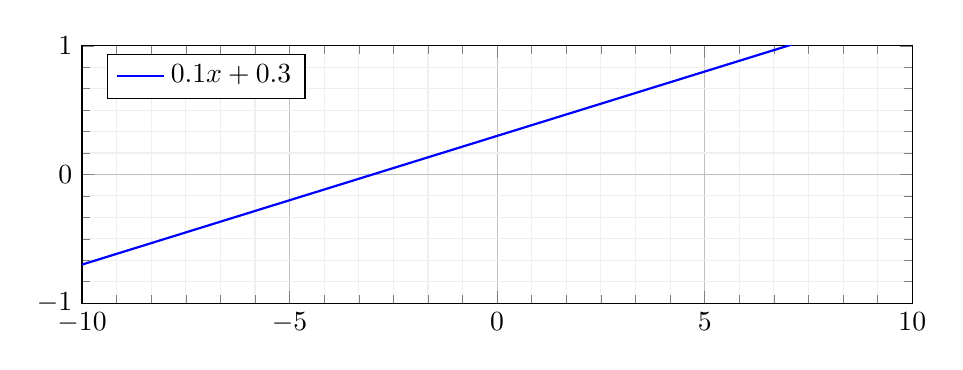
\begin{tikzpicture}
	
	\begin{axis}[
	xmin = -10, xmax = 10,
	ymin = -1, ymax = 1,
	xtick distance = 5,
	ytick distance = 1,
	grid = both,
	minor tick num = 5,
	major grid style = {lightgray},
	minor grid style = {lightgray!25},
	width = \textwidth,
	height = 0.4\textwidth,
	legend pos = north west
	]
	
	\addplot[
	domain = -10:10,
	samples = 200,
	smooth,
	thick,
	blue,
	] {0.1*x + 0.3};
	
	\legend{
		$0.1x + 0.3$, 
	}
	
	\end{axis}
	
	\end{tikzpicture}
	\caption{Linear function example}
\end{figure}

Suppose all neurons have linear activation functions. What is your neural network computing?

\end{frame}


\begin{frame}{Activation functions $\sigma$}
	
	Sigmoid (logistic) activation $\sigma(x) = \frac{1}{1 + \exp(-ax)}$
	
	\begin{figure}
		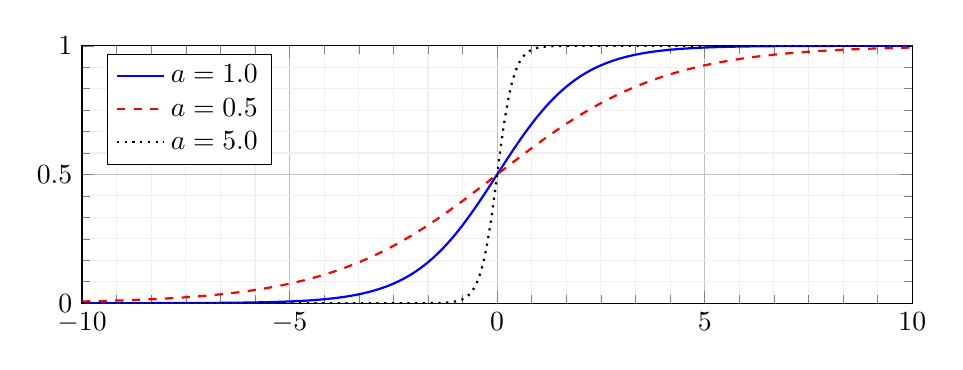
\begin{tikzpicture}
	
	\begin{axis}[
	xmin = -10, xmax = 10,
	ymin = 0, ymax = 1,
	xtick distance = 5,
	ytick distance = 0.5,
	grid = both,
	minor tick num = 5,
	major grid style = {lightgray},
	minor grid style = {lightgray!25},
	width = \textwidth,
	height = 0.4\textwidth,
	legend pos = north west
	]
	
	\addplot[
	domain = -10:10,
	samples = 200,
	smooth,
	thick,
	blue,
	] {1/(1 + exp(-1 * x))};
	
	\addplot[
	domain = -10:10,
	samples = 200,
	smooth,
	dashed,
	thick,
	red,
	] {1/(1 + exp(-0.5 * x))};
	
	\addplot[
	domain = -10:10,
	samples = 200,
	smooth,
	dotted,
	thick,
	black,
	] {1/(1 + exp(-5 * x))};
	
	\legend{
		$a = 1.0$, 
		$a = 0.5$,
		$a = 5.0$
	}
	
	\end{axis}
	
	\end{tikzpicture}
		\caption{Sigmoid function examples}
	\end{figure}
	
{\small Output not centered around $0$; gradient problematic for large values}	
\end{frame}

\begin{frame}{Activation functions $\sigma$}
	
	$\tanh$ activation
	
	\begin{figure}
		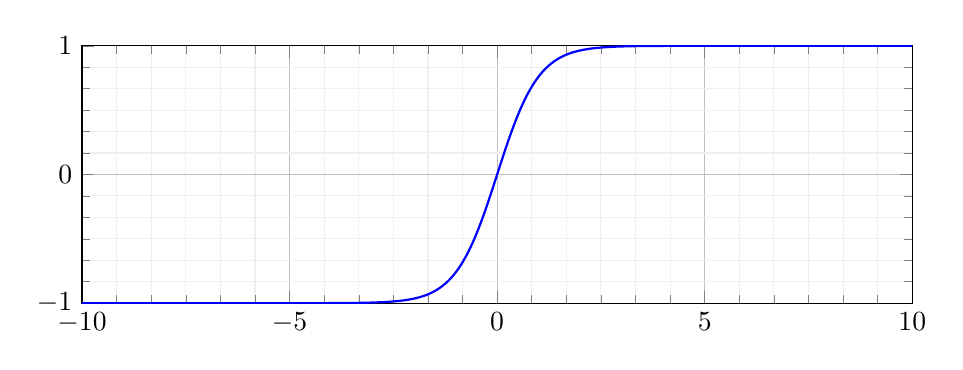
\begin{tikzpicture}
		
		\begin{axis}[
		xmin = -10, xmax = 10,
		ymin = -1, ymax = 1,
		xtick distance = 5,
		ytick distance = 1,
		grid = both,
		minor tick num = 5,
		major grid style = {lightgray},
		minor grid style = {lightgray!25},
		width = \textwidth,
		height = 0.4\textwidth,
		legend pos = north west
		]
		
		\addplot[
		domain = -10:10,
		samples = 200,
		smooth,
		thick,
		blue,
		] {tanh(x)};
		
	
		\end{axis}
		
		\end{tikzpicture}
		\caption{$\tanh$ function}
	\end{figure}
	
	{\small Centered around $0$; gradient problematic for large values}	
\end{frame}


\begin{frame}{Activation functions $\sigma$}
	
	Rectified linear unit (ReLU) activation
	
	\begin{columns}
		
	\begin{column}{0.6\linewidth}
		
		$$
		\mathrm{ReLU}(z) =
		\begin{cases}
		0  & \quad \text{if } z < 0\\
		z  & \quad \text{if } z \geq 0
		\end{cases}
		$$
	
	or \hspace{0.4em} $\mathrm{ReLU}(z) = \max(0, x)$
		
	{\small - Not centered around $0$; zero gradient problematic for negative values}	
	
	{\small - Gradient not saturate for positive values; Computationally efficient; Experimentally: converges faster}	
		
		
	\end{column}
	
	\begin{column}{0.4\linewidth}
	\begin{figure}
		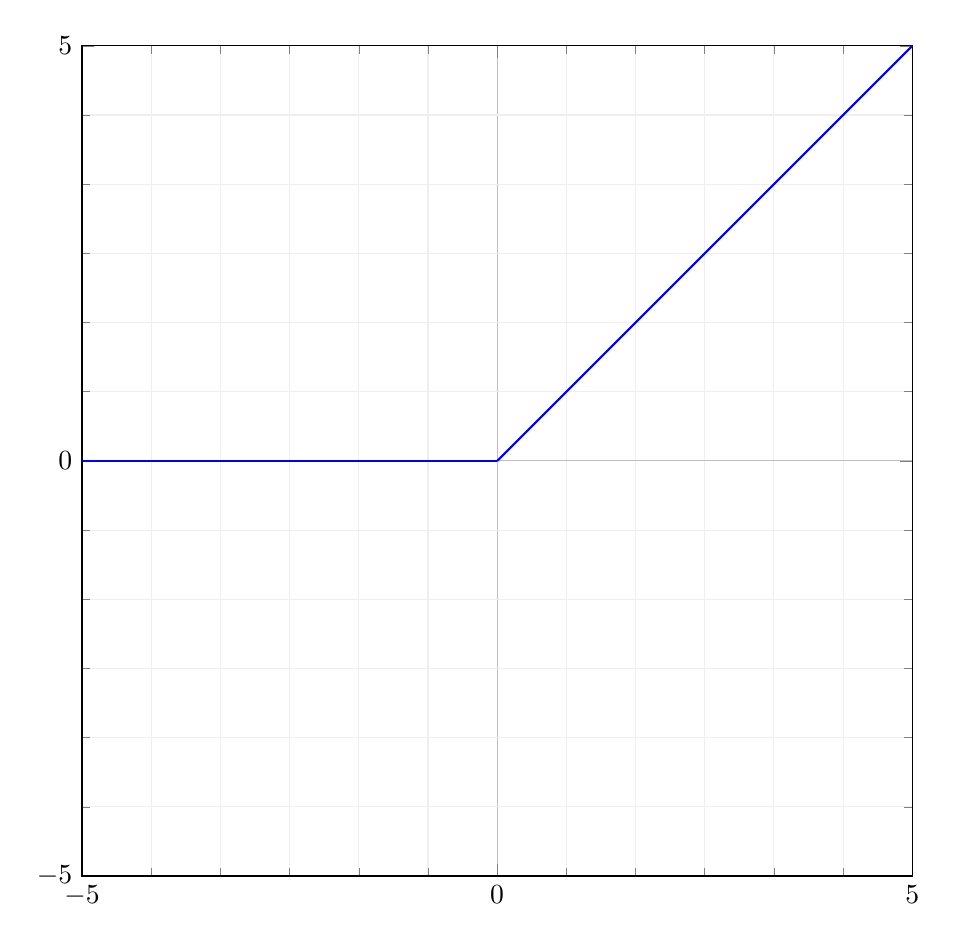
\begin{tikzpicture}
		
		\begin{axis}[
		xmin = -5, xmax = 5,
		ymin = -5, ymax = 5,
		xtick distance = 5,
		ytick distance = 5,
		grid = both,
		minor tick num = 5,
		major grid style = {lightgray},
		minor grid style = {lightgray!25},
		width = \textwidth,
		height = \textwidth,
		legend pos = north west
		]
		
		\addplot[
		domain = -5:0,
		samples = 10,
		smooth,
		thick,
		blue,
		] {0};
		
		\addplot[
		domain = 0:5,
		samples = 10,
		smooth,
		thick,
		blue,
		] {x};
		
		
		\end{axis}
		
		\end{tikzpicture}
		\caption{ReLU function}
	\end{figure}
		\end{column}
		\end{columns}
	

\end{frame}



\begin{frame}{Activation functions $\sigma$}
	
	Leaky ReLU activation
	
	\begin{columns}
		
		\begin{column}{0.6\linewidth}
			
			$$
			\mathrm{ReLU}(z) = \max(0.01x, x)
			$$
			
			{\small - Not entered around $0$}	
			
			{\small - Gradient O.K. for entire domain; Computationally efficient; Experimentally: converges fast}	
			
			
		\end{column}
		
		\begin{column}{0.4\linewidth}
			\begin{figure}
				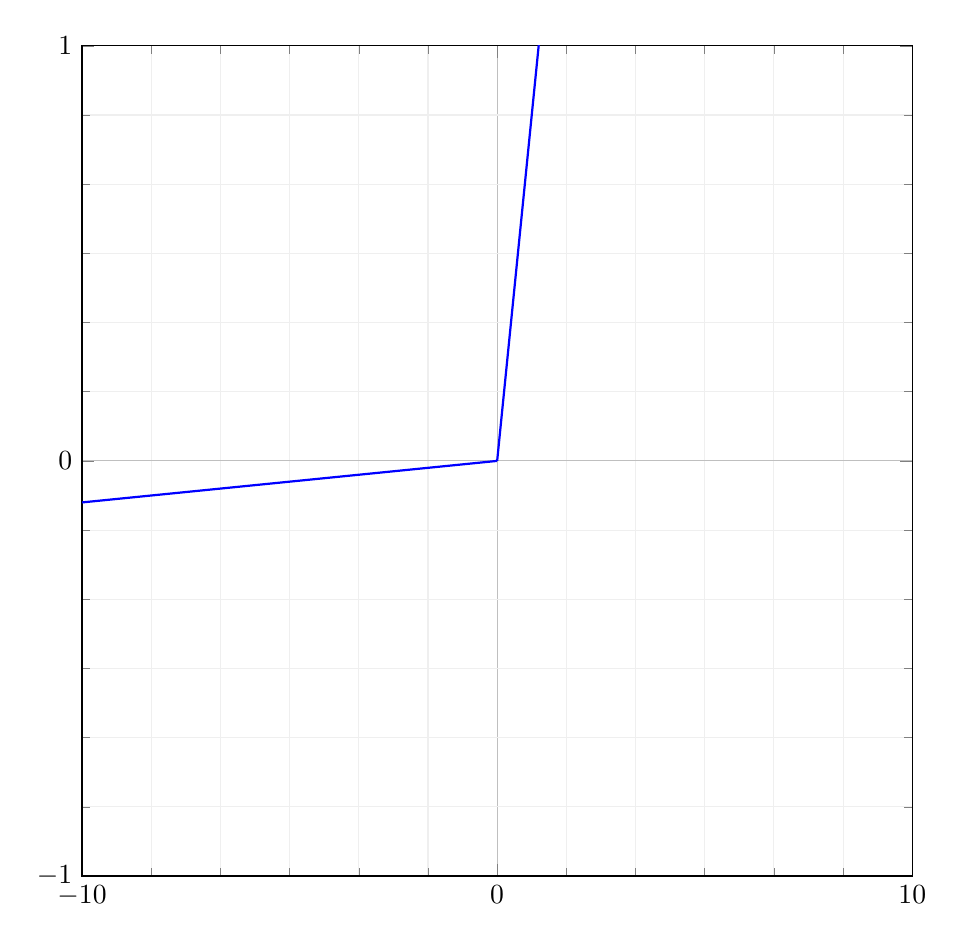
\begin{tikzpicture}
				
				\begin{axis}[
				xmin = -10, xmax = 10,
				ymin = -1, ymax = 1,
				xtick distance = 10,
				ytick distance = 1,
				grid = both,
				minor tick num = 5,
				major grid style = {lightgray},
				minor grid style = {lightgray!25},
				width = \textwidth,
				height = \textwidth,
				legend pos = north west
				]
				
				\addplot[
				domain = -10:0,
				samples = 10,
				smooth,
				thick,
				blue,
				] {0.01*x};
				
				\addplot[
				domain = 0:10,
				samples = 10,
				smooth,
				thick,
				blue,
				] {x};
				
				
				\end{axis}
				
				\end{tikzpicture}
				\caption{Leaky ReLU function}
			\end{figure}
		\end{column}
	\end{columns}
	
	
\end{frame}


\begin{frame}{A special activation function: softmax}


\begin{columns}[T,onlytextwidth]
	\column{0.5\linewidth}
	
	% move to the left by 3 em
	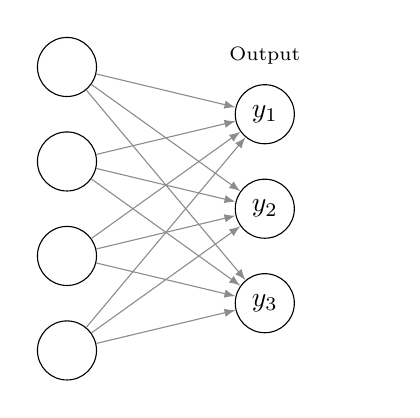
\begin{tikzpicture}
	\begin{scope}[node distance=1.5cm] % 2cm in general, 3.5cm for backprop task
	\matrix[layer] (input) {
		\\
		\\
		\\
		\\
	};
	
	\matrix[layer, right=of input] (output) {
		$y_1$ \\
		$y_2$ \\
		$y_3$ \\		
	};
	
	% dense layer connections
	\begin{scope}[thin, black!45, ->, >=latex]
	% input -> output
	\foreach \in in {1,2,3,4} {
		\foreach \done in {1,2,3} {
			\draw (input-\in-1) -- (output-\done-1);
		}
	}
	
	\end{scope}
	
	
	% layer descriptions
	\begin{scope}[every node/.style={align=center,text width=3cm}]
	\node[above=0cm of output] (outputdsc) {\scriptsize Output};
	\end{scope}
	
	\end{scope}
	\end{tikzpicture}
	
	\column{0.5\linewidth}
	
	Classification into multiple output classes (e.g., „Positive“, „Negative“, „Neutral“), we'd often like our outputs to represent a probability distribution over these classes
	
	$$y_1 + y_2 + y_3 = 1; \quad y_j \geq 0$$
	
\end{columns}

\end{frame}


\begin{frame}{A special activation function: softmax}
	
	
	\begin{columns}[T,onlytextwidth]
		\column{0.5\linewidth}
		
		% move to the left by 3 em
		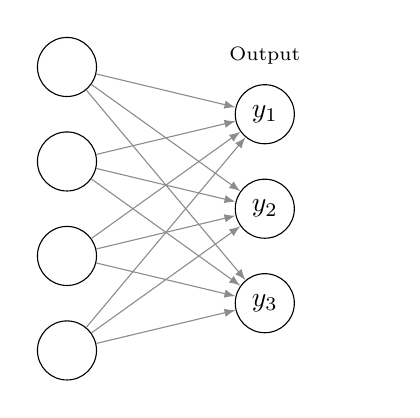
\begin{tikzpicture}
		\begin{scope}[node distance=1.5cm] % 2cm in general, 3.5cm for backprop task
		\matrix[layer] (input) {
			\\
			\\
			\\
			\\
		};
		
		\matrix[layer, right=of input] (output) {
			$y_1$ \\
			$y_2$ \\
			$y_3$ \\		
		};
		
		% dense layer connections
		\begin{scope}[thin, black!45, ->, >=latex]
		% input -> output
		\foreach \in in {1,2,3,4} {
			\foreach \done in {1,2,3} {
				\draw (input-\in-1) -- (output-\done-1);
			}
		}
		
		\end{scope}
		
		
		% layer descriptions
		\begin{scope}[every node/.style={align=center,text width=3cm}]
		\node[above=0cm of output] (outputdsc) {\scriptsize Output};
		\end{scope}
		
		\end{scope}
		\end{tikzpicture}
		
		\column{0.5\linewidth}
		
		Let $z_1$ be pre-activation of output node $y_1$
		
		$$
		y_1 = \frac{\exp(z_1)}{\exp(z_1) + \exp(z_2) + \exp(z_3)}
		$$
		
		For $m$ output nodes, \textbf{softmax} for each output node $y_j$ is
		
		$$
		y_j = \frac{\exp(z_j)}{\sum_{i = 1}^{m} \exp(z_i)}
		$$
		
	\end{columns}
	
\end{frame}



\begin{frame}{A special activation function: softmax}
	
\textbf{softmax} for each output node $y_j$ in a layer is

$$
y_j = \frac{\exp(z_j)}{\sum_{i = 1}^{m} \exp(z_i)}
$$

Unlike other activation functions, \textbf{softmax} depends on all units in the layer

- Global view, probabilistic interpretation
		
- Softmax name is misleading: It is not a smooth maximum but rather smooth approximation of \texttt{arg max} function (for soft maximum see \texttt{LogSumExp})


\end{frame}

\begin{frame}{Wrap up}
	
We started with organizational stuff

Then looked at the history of deep learning

.. and the history of NLP, as well as of problems in NLP (these are also historically changing!)

Afterwards, we presented the perceptron

Derived a learning algorithm

Finally, we looked at some basics of deep learning

\end{frame}

\begin{frame}[allowframebreaks]{References}

\printbibliography

%  \bibliography{demo}
%  \bibliographystyle{abbrv}

\end{frame}

\end{document}

